\section{Gravitational Fields}

\subsection{gravitational forces}

\subsubsection{Newton's law of gravitation}

any object attracts any other object through the gravitational force

\begin{figure}[ht]
	\centering
	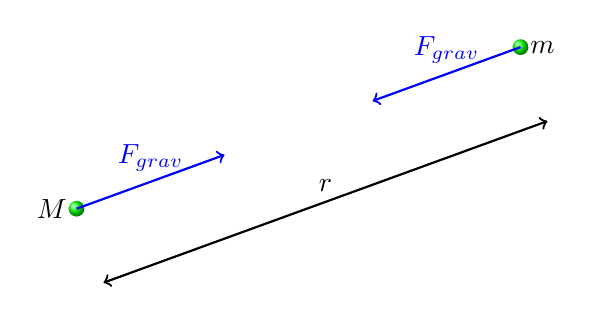
\begin{tikzpicture}[scale=1, rotate=20]
	\shade [ball color = green] (-3,0) node[left]{$M$} circle (0.1);
	\shade [ball color = green] (3,0) node[right]{$m$} circle (0.1);
	\draw [thick, <->] (-3,-1) -- (0,-1) node[above]{$r$} --(3,-1);
	\draw [thick,blue,->] (3,0) -- (2,0) node[above]{$F_\text{grav}$} --(1,0);
	\draw [thick,blue,->] (-3,0) -- (-2,0) node[above]{$F_\text{grav}$} --(-1,0);
	\end{tikzpicture}
	
	\caption*{gravitational attraction between $M$ and $m$}
	
	\vspace*{-15pt}
\end{figure}

\begin{ilight}
	\keypoint{Newton's law of gravitation}\index{Newton's law of gravitation} states that gravitational force between two \emph{point} masses is proportional to the product of their masses and inversely proportional to the square of their distance $\left(F_\text{grav} \propto \frac{Mm}{r^2}\right)$
\end{ilight}

this law was formulated in \emph{Issac Newton}'s work `The Principia', or `Mathematical Principles of Natural Philosophy', first published in 1687

mathematically, gravitational force takes the form: $\boxed{F_\text{grav}=\frac{GMm}{r^2}}$

$G = 6.67 \times 10^{-11} \text{ N m}^2 \text{ kg}^{-2}\,$ is the \emph{gravitational constant}

\cmt gravitational force is always \emph{attractive}

\cmt gravity is \emph{universal}, i.e., gravitational attraction acts between \emph{any} two masses

\cmt Newton's law of gravitation refers to \emph{point masses}

i.e., particles with no size, therefore distance $r$ can be easily defined

\begin{wrapfigure}{r}{5.4cm}
	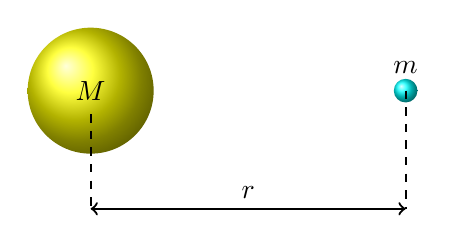
\begin{tikzpicture}[scale=1]
	\shade [ball color = yellow] (-2,0) node{$M$} circle (0.8);
	\shade [ball color = cyan] (2,0) circle (0.15);
	\node[above] at (2, 0.1) {$m$};
	\draw [thick, <->] (-2,-1.5) -- (0,-1.5) node[above]{$r$} --(2,-1.5);
	\draw [thick,dashed] (-2,-0.3) -- (-2,-1.5);
	\draw [thick,dashed] (2,0) -- (2,-1.5);
	\end{tikzpicture}
	
\end{wrapfigure}

\cmt a sphere with uniform mass distribution (e.g., stars, planets) can be treated as a \emph{point model}

distance $r$ is taken between centres of the spheres
\footnote{This is known as \emph{shell theorem}: a spherically symmetric shell (i.e., a hollow ball) affects external objects gravitationally as though all of its mass were concentrated at its centre, and it exerts no net gravitational force on any object inside, regardless of the object's location within the shell. ($\ast$)}

(see Example \ref{uniform-grav-field}, field lines around a planet \emph{seem} to point towards centre of planet)



\example{The Earth can be thought as a uniform sphere of radius $R = 6.4 \times 10^6$ m  and mass $M = 6.0 \times 10^{24}$ kg. Estimate the gravitational force on a man of 60 kg at sea level.}

\solc \begin{equation*}
F = \frac{GMm}{R^2} = \frac{6.67\times10^{-11}\times6.0\times10^{24}\times60}{(6.4\times10^6)^2} \approx 586 \text{ N} \teoe
\end{equation*}

\question{Estimate the gravitational force between you and your deskmate.}


\subsubsection{planetary motion}

\begin{figure}[ht]
	\centering
	\vspace*{-10pt}
	\begin{tikzpicture}
	\draw[dashed] (0,0) circle(2);
	\shade [ball color = yellow] (0,0) node[left]{$M$} circle (0.1);
	\shade [ball color = cyan] (30:2) node[right]{$m$} circle (0.1);
	\draw[thick,blue,->] (30:2) -- ++(210:1) node[below]{$F_\text{grav}$};
	\end{tikzpicture}
	
	\caption*{a planet/satellite orbiting around a star/earth}
	
	\vspace*{-10pt}
\end{figure}

a planet/satellite can move around a star/earth in circular orbit

circular motion requires centripetal force

for these objects, gravitational force provides centripetal force\vspace*{2pt}
\begin{equation*}
F_\text{grav} = F_c \RA
\boxed{\frac{GMm}{r^2} = \frac{mv^2}{r}} \quad \text{or} \quad \boxed{\frac{GMm}{r^2} = m \omega^2 r}
\end{equation*}

\vspace*{2pt}
\example{GPS (Global Positioning System) satellites move in a circular orbits at about 20000 km above the earth's surface. The Earth has a radius $R = 6.4 \times 10^6$ m  and mass $M = 6.0 \times 10^{24}$ kg. (a) Find the speed of GPS satellites. (b) Find its orbital period.}

\solc
\begin{equation*}
\frac{GMm}{r^2} = \frac{mv^2}{r} \RA v = \sqrt{\frac{GM}{r}} = \sqrt{\frac{6.67\times10^{-11}\times6.0\times10^{24}}{6.4\times10^6+2.0\times10^7}} \approx 3.9\times10^3 \mps
\end{equation*}
\begin{equation*}
v = \frac{2\pi r}{T} \RA T = \frac{2\pi r}{v} = \frac{2\pi\times(6.4\times10^6+2.0\times10^7)}{3.9\times10^3} \approx 4.3\times10^4 \text{ s} \approx 11.8 \text{ hours} \teoe
\end{equation*}

\example{A \keypoint{geostationary satellite} \index{geostationary orbit} moves in a circular orbit that appears motionless to ground observers. The satellite follows the Earth's rotation, so the satellite rotates from west to east above equator with an orbital period of 24 hours. Find the radius of this orbit.} 

\solc
\begin{equation*}
\frac{GMm}{r^2} = m \omega^2 r \RA \frac{GMm}{r^2} = m\left(\frac{2\pi}{T}\right)^2 r \RA r^3 = \frac{GMT^2}{4\pi^2}
\end{equation*}
\begin{equation*}
r = \left( \frac{GMT^2}{4\pi^2} \right)^{1/3} = \left( \frac{6.67\times10^{-11} \times 6.0\times10^{24} \times (24\times3600)^2}{4\pi^2} \right)^{1/3} \approx 4.23\times10^7 \text{ m} \teoe
\end{equation*}

\example{Assuming the planets in the solar system all move around the sun in circular orbits, show that the square of  orbital period is proportional to the cube of orbital radius.
	\footnote{This is known as \emph{Kepler's 3rd law} for planetary motions. In the early 17th century, German astronomer Johannes Kepler discovered three scientific laws which describes how planets move around the sun. This $T^2 \propto r^3$ relation not only holds for circular orbits but are also correct for elliptical orbits.
		
		Isaac Newton proved that Kepler's laws are consequences of his own law of universal gravitation, and therefore explained why the planets move in this way.}}

\solc
\begin{equation*}
\frac{GMm}{r^2} = m \omega^2 r \RA \frac{GMm}{r^2} = m\left(\frac{2\pi}{T}\right)^2 r \RA T^2 = \frac{4\pi^2}{GM}\cdot r^3
\end{equation*}

$G$ is gravitational constant, $M$ is mass of the sun, so $\frac{4\pi^2}{GM}$ is a constant, so $T^2 \propto r^3$ \eoe

\question{Given that it takes about 8.0 minutes for light to travel from the sun to the earth. (a) What is the mass of the sun? (b) At what speed does the earth move around the sun?}

\subsubsection{apparent weight}

an object's \emph{actual weight} is the gravitational attraction exerted by the
earth's gravity

an object's \emph{apparent weight} is the upward force (e.g., normal contact force exerted by ground, tension in a spring balance, etc.) that opposes gravity and prevents the object from falling

apparent weight can be different from actual weight due to vertical acceleration or buoyancy

but if we consider rotation of the earth, this also causes apparent weight to be lessened

\begin{figure}[ht]
	\centering
	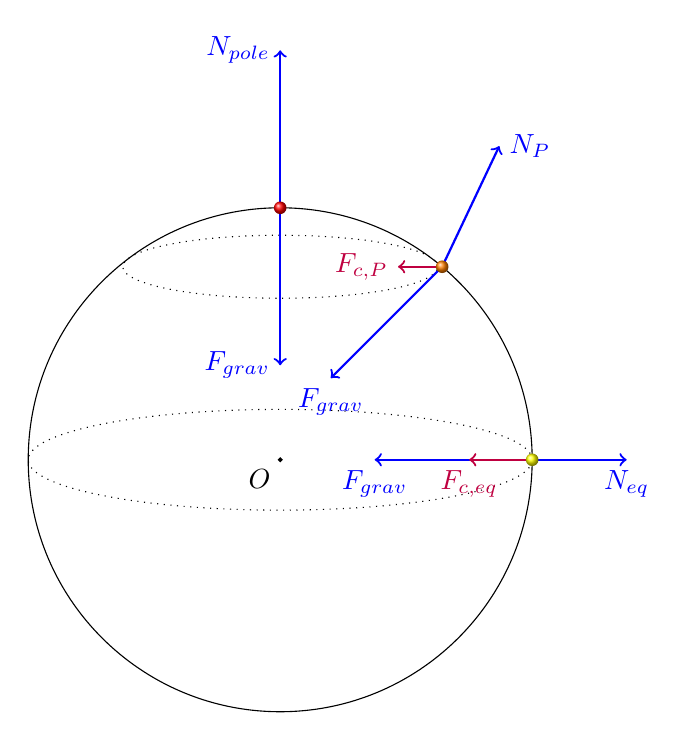
\begin{tikzpicture}[scale=0.8]
	\draw (0,0) node[below left]{$O$} circle(4);
	\draw[fill] (0,0) circle(0.03);
	\draw[dotted] (0,0) ellipse (4 and 0.8);
	\draw[dotted] (0,3.064) ellipse (2.5 and 0.5);
	\draw[thick,blue,->] (4,0) --++ (-2.5,0) node[below]{$F_\text{grav}$};
	\draw[thick,blue,->] (4,0) --++ (1.5,0) node[below]{$N_\text{eq}$};
	\draw[thick,purple,->] (4,0) --++ (-1,0) node[below]{$F_{c,\text{eq}}$};
	\draw[thick,blue,->] (50:4) --++ (225:2.5) node[below]{$F_\text{grav}$};
	\draw[thick,purple,->] (50:4) --++ (-0.7,0) node[left]{$F_{c,P}$};
	\draw[thick,blue,->] (50:4) --++ (0.907,1.915) node[right]{$N_P$};
	\draw[thick,blue,->] (0,4) --++ (0,-2.5) node[left]{$F_\text{grav}$};
	\draw[thick,blue,->] (0,4) --++ (0,2.5) node[left]{$N_\text{pole}$};
	\shade [ball color = yellow] (4,0) circle (0.1);
	\shade [ball color = orange] (50:4)  circle (0.1);
	\shade [ball color = red] (90:4) circle (0.1);
	\end{tikzpicture}
	
	apparent weight at various positions near earth's surface (not to scale)
\end{figure}

object resting on ground is actually rotating together with earth

resultant of gravitational force and contact force should provide centripetal force

for object on equator: $F_{c,\text{eq}} = m\omega^2 R \RA F_\text{grav} - N_\text{eq} = m \omega^2 R  \RA N_\text{eq} = \frac{GMm}{R^2} - m \omega^2 R$

for object at poles: $F_{c,\text{pole}} = 0 \RA F_\text{grav} - N_\text{pole} = 0  \RA N_\text{pole} = \frac{GMm}{R^2}$

at lower latitudes, object describe larger circles, hence requires greater centripetal force

this offsets the balancing normal force, so apparent weight decreases near the equator

\example{A stone of mass 5.0 kg is hung from a newton-meter near the equator. The Earth can be considered to be a uniform sphere of radius $R = 6370$ km  and mass $M = 5.97 \times 10^{24}$ kg. (a) What is the gravitational force on the stone? (b) What is the reading on the meter?}

\sol gravitational force: $F_\text{grav} = \frac{GMm}{R^2} = \frac{6.67\times10^{-11}\times5.97\times10^{24}\times5.0}{(6.37\times10^6)^2} \approx 49.07 \text{ N}$

centripetal force required: $F_c = m\omega^2 R = m\left(\frac{2\pi}{T}\right)^2R = 5.0\times\frac{4\pi^2}{(24\times3600)^2}\times6.37\times10^6 \approx 0.17 \text{ N}$

apparent weight, or reading on meter: $N = F_\text{grav} - F_c = 49.07 - 0.17 \approx 48.90 \text{ N}$ \eoe

\question{Why astronauts in space stations are said to be \emph{weightless}?}

\question{How do you find the apparent weight of an object at an arbitrary latitude $P$? Does the apparent weight act vertically downwards? Give your reasons.}


\subsection{gravitational fields}

to explain how objects exert gravitational attraction upon one another at a distance, we introduce the concept of \emph{force fields}

\begin{ilight}
	\keypoint{gravitational field} is a region of space where a mass is acted by a force
\end{ilight}

any mass $M$ (or several masses) can produce a gravitational field around it

a test mass $m$ within this field will experience a gravitational force

\vspace*{\baselineskip}

to describe the effect on a small mass $m$ in the field, we will further introduce
\begin{itemize}
	\item[-] \emph{gravitational field strength}, to help us compute gravitational force on objects
	
	\item[-] \emph{gravitational potential}, to help us compute gravitational potential energy between objects
\end{itemize}


\subsection{gravitational field strength}

\subsubsection{gravitational field strength}

\rcyskip

\begin{ilight}
	\keypoint{gravitational field strength}\index{gravitational field!gravitational field strength} is defined as gravitational force per unit mass: $\boxed{g=\frac{F_\text{grav}}{m}}$
\end{ilight}

\cmt unit of $g$: $[g]=\text{N kg}^{-1} = \mpss$, same unit as acceleration

\cmt field strength due to an isolated source of mass $M$

at distance $r$ from the source, a test mass $m$ is acted by a force: $F_\text{grav} = \frac{GMm}{r^2}$

field strength at this position: $g = \frac{F_\text{grav}}{m} = \RA \boxed{g=\frac{GM}{r^2}}$

note that the field is produced by the source $M$, so field strength $g$ depends on $M$, not $m$

\cmt field strength $g$ is a \emph{vector} quantity, it has a direction

gravitation is \emph{attractive}, so $g$ points towards source mass

to compute combined field strength due to several sources, should perform \emph{vector sum} of contributions from each individual

\example{Star $A$ of mass $6.0\times10^{30} \text{ kg}$ and star $B$ of mass $1.5\times10^{30} \text{ kg}$ are separated by a distance of $2.0 \times 10^{12} \text{ m}$. (a) What is the field strength at the mid-point $P$ of the two stars? (b) If a comet of mass $4.0\times10^6 \text{ kg}$ is at the mid-point, what force does it experience?}

\begin{center}
	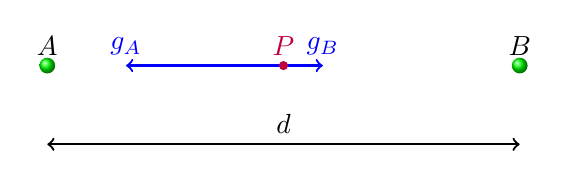
\begin{tikzpicture}
		\shade [ball color = green] (-3,0) node[above]{$A$} circle (0.1);
		\shade [ball color = green] (3,0) node[above]{$B$} circle (0.1);
		\draw [thick, <->] (-3,-1) --(3,-1) node[above, midway]{$d$};
		\draw [thick,blue,->] (0,0) -- (-2,0) node[above]{$g_A$};
		\draw [thick,blue,->] (0,0) -- (0.5,0) node[above]{$g_B$};
		\draw[fill,purple] (0,0) circle(0.05) node[above]{$P$};
	\end{tikzpicture}
\end{center}

\sol $g_A$ acts towards $A$, $g_B$ acts towards $B$, they are in opposite directions
\begin{equation*}
	g_P = g_A - g_B = \frac{GM_A}{r_A^2} - \frac{GM_B}{r_B^2} = 6.67\times10^{-11} \times\left[ \frac{6.0\times10^{30}}{(1.0\times10^{12})^2} - \frac{1.5\times10^{30}}{(1.0\times10^{12})^2}\right] \approx 3.0\times10^{-4} \text{ N kg}^{-1}
\end{equation*}

force on comet: $F=mg = 4.0\times10^6 \times 3.0\times10^{-4} \approx 1.2\times10^3 \text{ N}$ \eoe

\subsubsection{acceleration of free fall}

if field strength $g$ is known, gravitational force on an object of mass $m$ is: $F_\text{grav} = mg$

if the object is acted by gravity only, then $\fnet = F_\text{grav} \RA ma = mg \RA \boxed{a=g}$
\footnote{Rigorously speaking, the two $m$'s are different concepts. There is the \emph{inertia} mass, decribing how much an object resists the change of state of motion. There is also the \emph{gravitational} mass, describing the effect produced and experienced by the object in gravitational fields. Yet no experiment has ever demonstrated any significant difference between the two. The reason why the two masses are identical is very profound. We have shown here acceleration of free fall equals gravitational field strength, but Albert Einstein's \emph{equivalence principle} suggests that it is actually impossible to distinguish between a uniform acceleration and a uniform gravitational field. This idea lies at the heart of the \emph{general theory of relativity}, where I should probably stop going further.}

this shows gravitational field strength gives the acceleration of free fall!

\example{The earth has a radius of 6370 km. (a) Find the mass of the earth.
	\footnote{British scientist Henry Cavendish devised an experiment in 1798 to measure the gravitational force between masses in his laboratory. He was the first man to yield accurate values for the gravitational constant $G$. Then he was able to carry out this calculation, referred by himself as `weighing the world'.} 
(b) Find the acceleration of free fall at the top of Mount Everest. (height of Mount Everest $H\approx 8.8 \text{ km}$)}

\sol consider acceleration of free fall near surface of earth:
\begin{equation*}
	g_s = \frac{GM}{R^2} \RA 9.81 = \frac{6.67\times10^{-11}\times M}{(6.37\times10^6)^2} \RA M \approx 5.97\times10^{24} \text{ kg}
\end{equation*}

at top of Mount Everest:
\begin{equation*}
g_\text{ME} = \frac{GM}{(R+H)^2} = \frac{6.67\times10^{-11}\times 5.97\times10^{24}}{(6.37\times10^6+8.8\times10^3)^2} \approx 9.78 \text{ N kg}^{-1} \RA a_\text{ME} \approx 9.78 \mpss \teoe
\end{equation*}



\subsubsection{gravitational field lines}
\keypoint{gravitational field lines}\index{field line!gravitaional field line} are drawn to graphically represent the pattern of field strength

\cmt \emph{direction} of field lines show the \emph{direction} of field strength in the field
	
\cmt \emph{spacing} between field lines indicates the \emph{strength} of the gravitational field
	
\cmt gravitational field lines always end up at a mass

     this arises from the attractive nature of gravitation

\noindent\begin{minipage}[t]{0.48\textwidth}
		\example{field around the earth}\label{uniform-grav-field}
			\begin{center}
				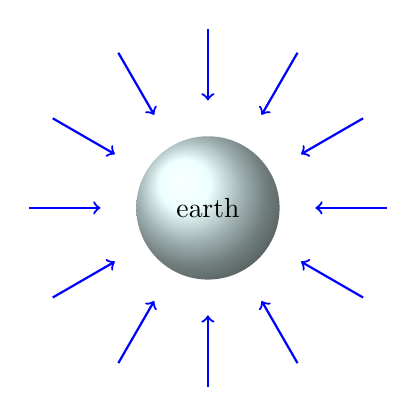
\begin{tikzpicture}[scale=0.91]
				\shade [ball color = cyan!10] (0,0) node{earth} circle [radius=1];
				\foreach \s in {0,30,60,...,330}
				\draw [blue, thick, <-] (\s:1.5) -- ++(\s:1);
				\end{tikzpicture}
				
				\emph{radial} field (field lines normal to surface)
			\end{center}
	\end{minipage}
	\begin{minipage}[t]{0.5\textwidth}
		\example{field near earth's surface}
			\begin{center}
				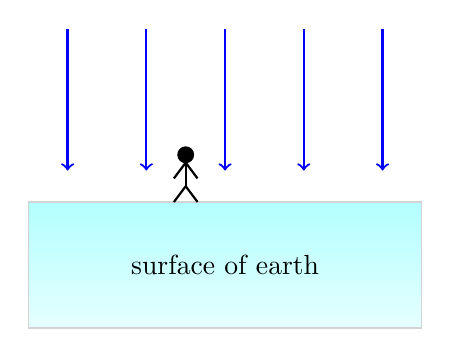
\begin{tikzpicture}[scale=1]
				\foreach \s in {-2,-1,0,1,2}
				\draw [blue, thick, <-] (\s,1.2) -- (\s,3);
				\draw[LightGrey,shade,
				top color=Cyan!30,
				bottom color=cyan!10] (-2.5,-0.8) rectangle (2.5,0.8);
				\draw (0,0) node{surface of earth};
				\draw [fill=black](-0.5,1.4) circle[radius=0.1];
				\draw [thick] (-0.5,1.4) -- (-0.5,1.0);
				\draw [thick] (-0.35,0.8) -- (-0.5,1.0);
				\draw [thick] (-0.65,0.8) -- (-0.5,1.0);
				\draw [thick] (-0.35,1.1) -- (-0.5,1.3);
				\draw [thick] (-0.65,1.1) -- (-0.5,1.3);
				\end{tikzpicture}
				
				almost a \emph{uniform} field
				
				(field lines are parallel and equally spaced)
			\end{center}
	\end{minipage}




\subsection{gravitational potential \& potential energy}

\subsubsection{potential energy}

\emph{potential energy} is the energy possessed by an object due to its position in a force field

work done \emph{by} force field decreases P.E., and work done \emph{against} a force field increases P.E.

let $W$ be work by the force field, then we have: $\boxed{W=-\Delta E_p}$

\newpage

to define potential energy of an object at a specific point $X$, we can

\begin{compactenum}
	\item[(1)] choose a position where potential energy is defined to be zero
	
	\item[(2)] find work done by force field to bring the object from zero P.E. point to $X$
	
	\item[(3)] consider change in P.E.: $\Delta E_p = E_{p,X} - E_{p,\text{initial}} = E_{p,X} - 0 = E_{p,X}$
	
	but $\Delta E_p = -W$, so P.E. at point $X$ is found: $E_{p,X} = -W$
	
\end{compactenum}

so potential energy is equal to (negative) work done to move the object to a specific position

\subsubsection*{gravitational potential energy near earth's surface}

we may choose a zero G.P.E. point, for example, $E_p(0) = 0$ at sea level

if mass $m$ is moved up for a height $h$, work done by gravity is $W=-mgh$\footnote{Negative sign because this is work against gravity.}

this causes a change in gravitational potential energy $\Delta E_p=-W=mg h$

then at altitude $h$, G.P.E. can be given by $E_p(h)=mgh$

\subsubsection{gravitational potential energy}


we are now ready to derive an expression for G.P.E. between two masses $M$ and $m$

we define $E_p=0$ at $r=\infty$ (choice of zero potential energy, no force so no G.P.E.), then

\begin{ilight}
	\keypoint{gravitation potential energy} is equal to the work done by gravitational force to bring a mass to a specific position from \emph{infinity}
\end{ilight} 

consider a mass $m$ at infinity with zero energy and a source mass $M$ at origin

let's find out how much work is done by gravitational force to pull $m$ towards the origin

\begin{center}
	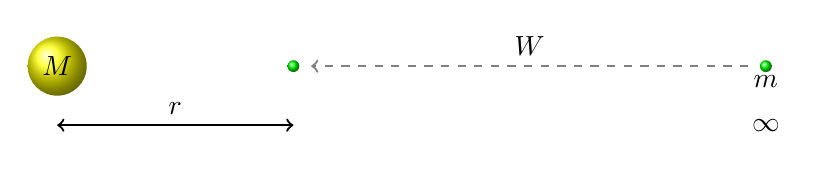
\begin{tikzpicture}[scale=0.75]
	\shade [ball color = yellow] (-4,0) node{$M$} circle [radius=0.5];
	\shade [ball color = green] (8,0) node[below]{$m$} circle [radius=0.1];
	\draw [thick, <->] (0,-1) -- (-2,-1) node[above]{$r$} --(-4,-1);
	\draw [thick,dashed,gray,->] (7.7,0) -- (0.3,0) node[midway,above]{\textcolor{black}{$W$}};
	\shade [ball color = green] (0,0) circle [radius=0.1];
	\draw (8,-1) node{$\infty$};
	\end{tikzpicture}
\end{center}

\begin{figure}[ht]
	\centering
%	\vspace*{-5pt}
	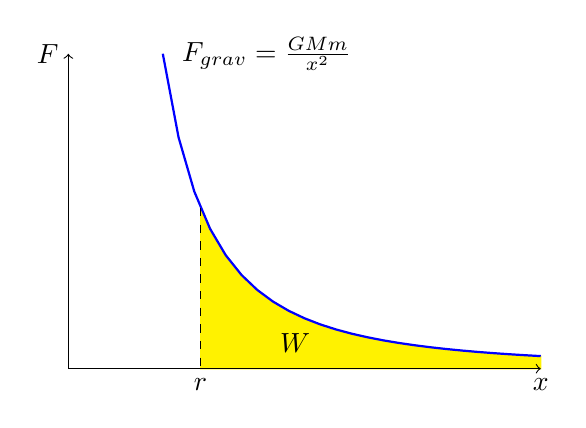
\begin{tikzpicture}[xscale=1.2]
	\draw [yellow,fill,domain=1.4:5] (1.4,2.04) -- plot (\x, 4/\x/\x) -- (5,0) -- (1.4,0) -- cycle;
	\draw[<->] (0,4) node[left]{$F$} -- (0,0) -- (5,0) node[below]{$x$};
	\draw [thick,domain=1:5,blue] plot (\x, 4/\x/\x);
	\draw[dashed] (1.4,2.04) -- (1.4,0) node[below]{$r$};
	\node at (2.4,0.33) {$W$};
	\node[right] at (1.1,4) {$F_\text{grav}=\frac{GMm}{x^2}$};
	\end{tikzpicture}
\end{figure}

but $F_\text{grav}$ varies as inverse square of separation $x$

so here we need to evaluate work done by a non-constant force

we can plot a $F$-$x$ graph, then magnitude of work done equals area under the graph

integrate\footnote{In general, work done by a non-constant force over large distance is $W = \int_\text{initial}^\text{final} F \dd x $.
	
For our case, $x$ is the displacement away from the source, but gravitational force tends to pull the mass towards the source. $F$ and $x$ are in opposite directions, a negative sign is needed for $F$. Therefore the work done by gravity to bring mass $m$ from infinity is: $W = \int_\infty^r F \dd x = \int_\infty^r \left(-\frac{GMm}{x^2}\right)\dd x = +\frac{GMm}{x} \Bigg|_\infty^r = \frac{GMm}{r}$.} to evaluate the area: $W = \int_r^\infty \frac{GMm}{x^2} \dd x = - \frac{GMm}{x}\Bigg|^\infty_r = \frac{GMm}{r}$


$\Delta E_p = -W \RA E_p(r) - E_p(\infty) = - \frac{GMm}{r}$

but we have defined $E_p(\infty)=0$, therefore: $\boxed{E_p(r)= -\frac{GMm}{r}}$

$E_p(r)$ gives G.P.E between masses $M$ and $m$ when they are at distance $r$ from each other

\cmt as $r \to \infty$, $E_p \to 0$, this agrees with our choice of zero G.P.E. point

\cmt potential energy is a \emph{scalar} quantity (negative sign cannot be dropped)

\cmt G.P.E. is always \emph{negative}, this is due to \emph{attractive} nature of gravity

to separate masses, work must be done to overcome attraction

so G.P.E. increases with separation $r$, i.e., G.P.E. is maximum at infinity, which is zero

G.P.E. between masses at finite separation must be less than zero

\cmt $E_p=mgh$ is only applicable near earth's surface where field is almost \emph{uniform}

$E_p =-\frac{GMm}{r}$ is a more \emph{general} formula for gravitational potential energy
\footnote{One can recover $\Delta E_p=mg\Delta h$ from $E_p=-\frac{GMm}{r}$. Near the earth's surface, if $r_1\approx r_2\approx R$, and $r_1>r_2$, then we have: $\Delta E_p = E_p(r_1) - E_p(r_2) = -GMm\left(\frac{1}{r_1}-\frac{1}{r_2}\right) = GMm \frac{r_1-r_2}{r_1r_2} \approx m \frac{GM}{R^2} \Delta r \xlongequal{g=GM/R^2} mg\Delta h$.}



\example{A meteor is travelling towards a planet of mass $M$. When it is at a distance of $r_1$ from centre of $M$, it moves at speed $v_1$. When it is $r_2$ from $M$, it moves at speed $v_2$. Assume only gravitational force applies, establish a relationship between these quantities.}

\sol energy conservation: $\text{K.E.} + \text{G.P.E.} = \text{const}$ $\ra$ $\frac{1}{2}mv_1^2+\left(-\frac{GMm}{r_1}\right) = \frac{1}{2}mv_2^2+\left(-\frac{GMm}{r_2}\right)$ \eoe

\example{If an object is thrown from the surface of a planet at sufficiently high speed, it might escape from the influence of the planet's gravitational field. The minimum speed required is called the \emph{escape velocity}\index{escape velocity}. Using the data from previous examples, find the escape velocity from the surface of earth.}
	
\sol assuming no energy loss to air resistance, then total energy is conserved
\begin{equation*}
	\text{K.E.} + \text{G.P.E. at surface of planet} = \text{K.E.} + \text{G.P.E. at infinity}
\end{equation*}
\begin{equation*}
	\frac{1}{2} mu^2 +\left(-\frac{GMm}{R}\right) = \frac{1}{2}mv^2 + 0 \quad \xLongrightarrow{v\geq 0} \quad u^2 \geq \frac{2GM}{R} \RA u_\tmin = \sqrt{\frac{2GM}{R}}
\end{equation*}

for earth, escape velocity $u_\tmin = \sqrt{\frac{2\times6.67\times10^{-11}\times6.0\times10^{24}}{6.4\times10^6}} \approx 1.12\times10^4\mps$ \eoe

%\question{A planet of uniform density distribution is of radius $R$ and mass $M$. A rock falls from a height of $3R$ above the surface of the planet. Assume the planet has no atmosphere, show that the speed of the rock when it hits the ground is $v=\sqrt{\frac{3GM}{4R}}$.} I think there is a typo for $v=\sqrt{\frac{3GM}{4R}}$, it should be $v=\sqrt{\frac{3GM}{2R}}$%

\question{A planet of uniform density distribution is of radius $R$ and mass $M$. A rock falls from a height of $3R$ above the surface of the planet. Assume the planet has no atmosphere, show that the speed of the rock when it hits the ground is $v=\sqrt{\frac{3GM}{2R}}$.}

\sol By energy conservation
$$
-\frac{G M m}{4 R}+0=-\frac{G M m}{R}+\frac{1}{2} m v^2 \q \Rightarrow \q v=\sqrt{\frac{3 G M}{2 R}}
$$



\question{A space probe is travelling around a planet of mass $M$ in a circular orbit of radius $r$. (a) Show that the total mechanical energy (sum of kinetic energy and gravitational energy) of the space probe is $E_\text{total} = -\frac{2GMm}{r}$. (b) If the space probe is subject to small resistive forces, state the change to its orbital radius and its orbiting speed.}


\sol (a) Orbit speed is given by and hence kinetic energy is
$$
v^2=\frac{G M}{r} \q \Rightarrow \q K E=\frac{1}{2} m\left(\frac{G M}{r}\right)=\frac{G M m}{2 r}
$$

so total mechanical energy is
$$
E_{\text {total }}=K E+P E=\frac{G M m}{2 r}-\frac{G M m}{r}=-\frac{G M m}{2 r}
$$

(b) The energy decreases due to resistive forces, therefore according to the expression of $E$, the radius will decrease. And since radius decreases, the orbiting speed will increase.

\question{A \emph{black hole} is a region of spacetime where gravitation is so strong that even light cannot escape from it. For a star of mass $M$ to collapse and form a black hole, it has to be compressed below a certain radius. (a) Show that this radius is given by $R_S = \frac{2GM}{c^2}$, known as the \emph{Schwarzschild radius}\footnote{When you deal with very strong gravitational fields, Newton's law of gravitation breaks down and effects of Einstein's \emph{general theory of relativity} come into play. The radius of a \emph{Newtonian} black hole being equal to the radius of a Schwarzschild black hole is a mere coincidence.}. (b) Show that the Schwarzschild radius for the sun is about 3 km.}

\sol (a) The Schwarzschild radius $R_S$ is the radius below which the escape velocity from the gravitational pull of an object exceeds the speed of light, $c$. The escape velocity $v_e$ is given by:
$$
v_e=\sqrt{\frac{2 G M}{r}}
$$

Setting $v_e=c$ :
$$
c=\sqrt{\frac{2 G M}{R_S}}
$$

Squaring both sides:
$$
c^2=\frac{2 G M}{R_S}
$$

Solving for $R_S$ :
$$
R_S=\frac{2 G M}{c^2}
$$

(b) Substitute the value, we can show that the radius is about 3 km.

\newpage

\subsubsection{gravitational potential}

it is useful to introduce a quantity called \emph{potential} at a specific point in a gravitational field

gravitational potential can be considered as the potential energy per unit mass: $\varphi = \frac{E_p}{m}$

\begin{ilight}
	\keypoint{gravitational potential}\index{gravitational field!gravitational potential} at a point is defined as the work done to bring \emph{unit} mass from \emph{infinity} to that point
\end{ilight}

\begin{wrapfigure}{r}{6cm}
	\centering
	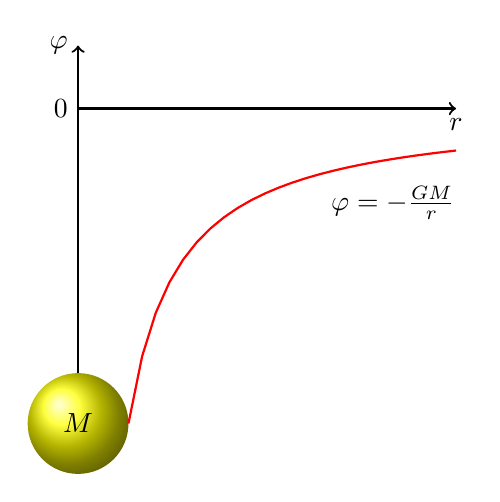
\begin{tikzpicture}[scale=0.8]
	\draw[thick,->] (0,0) node[left]{0} -- (6,0) node[below] {$r$};
	\draw[thick,->] (0,-5.5) -- (0,1) node[left]{$\varphi$};
	\shade [ball color = yellow] (0,-5) node{$M$} circle [radius=0.8];
	\draw[thick,red,domain=0.8:6,variable=\x] plot (\x,-4/\x);
	\node at (5,-1.5) {$\varphi = - \frac{GM}{r}$};
	\end{tikzpicture}
\end{wrapfigure}

\cmt unit: $[\varphi] = \text{J kg}^{-1}$

\cmt gravitational potential due to an isolated source $M$

{

\centering

$\varphi = \frac{E_p}{m} = \frac{-\frac{GMm}{r}}{m} \RA \boxed{\varphi = - \frac{GM}{r}}$

}

\cmt potential at infinity is zero: $\varphi_\infty = 0$

this is our choice of zero potential point

\cmt gravitational potential is a \emph{scalar}

combined potential due to several masses equals scalar sum of potential of each individual

\cmt gravitational potential is always \emph{negative}

again this arises from attractive nature of gravity

work is done to pull unit mass away from source

farther from source means higher potential

\example{A star $A$ of mass $M_A=1.5\times10^{30}$ kg and a planet $B$ of mass $M_B=6.0\times10^{26}$ kg form an isolated astronomical system. Point $P$ is between $A$ and $B$, and is at distance $r_A=2.0\times10^{12}$ m from $A$, and distance $r_B=8.0\times10^{10}$ m from $B$. (a) Find the gravitational potential at $P$. (b) A meteor is initially at very large distance from the system with negligible speed. It then travels towards point $P$ due to the gravitational attraction. Find its speed when it reaches $P$.}

\sol gravitational potential at $P$: $\, \varphi_P = \varphi_A + \varphi_B = \left(-\frac{GM_A}{r_A}\right) + \left(-\frac{GM_B}{r_B}\right)$
\begin{equation*}
\varphi_P = -6.67\times10^{-11}\times\left(\frac{1.5\times10^{30}}{2.0\times10^{12}} + \frac{6.0\times10^{26}}{8.0\times10^{10}}\right) \approx -5.05\times10^{7} \text{ J kg}^{-1}
\end{equation*}

gain in K.E. = loss in G.P.E.: $\, \frac{1}{2}mv^2 = m\Delta \varphi \RA v^2 = 2(\varphi_\infty - \varphi_P)=-2\varphi_P$
\begin{equation*}
v=\sqrt{-2\times(-5.05\times10^7)} \approx 1.01\times10^4 \mps \teoe
\end{equation*}

\example{The Moon may be considered to be an isolated sphere of radius $R=1.74 \times 10^3$ km. The gravitational potential at the surface of the moon is about $-2.82 \times 10^6 \text{ J kg}^{-1}$. (a) Find the mass of the moon. (b) A stone travels towards the moon such that its distance from the centre of the moon changes from $3R$ to $2R$. Determine the change in gravitational potential. (c) If the stone starts from rest, find its final speed.}

\sol at surface: $\varphi(R) = -\frac{GM}{R} \RA -2.82\times10^6 = -\frac{6.67\times10^{-11}\times M}{1.74\times10^6} \RA M = 7.36 \times 10^{22} \text{ kg}$

\eqyskip from $3R$ to $2R$: $\Delta \varphi = \varphi_{(3R)} - \varphi_{(2R)} = \left(-\frac{GM}{3R}\right) - \left(-\frac{GM}{2R}\right) = \frac{GM}{6R} = \frac{2.82\times10^6}{6} \approx 4.70 \times 10^5 \text{ J kg}^{-1}$

note this change is a \emph{decrease} in gravitational potential

gain in K.E. = loss in G.P.E.: $\, \frac{1}{2}mv^2 = m\Delta \varphi \RA v = \sqrt{2\Delta \varphi} = \sqrt{2\times4.70 \times 10^5} \approx 970 \mps$ \eoe

\question{Given that the moon is of radius 1700 km and mass $7.4\times10^{22}$ kg. (a) Find the change in gravitational potential when an object is moved from moon's surface to 800 km above the surface. (b) If a rock is projected vertically upwards with an initial speed of $1800\mps$ from surface, find the rock's speed when it reaches a height of 800 km. (c) Suggest whether the rock can escape from the moon's gravitational field completely.}
